\documentclass[12pt]{article}

\usepackage{ctex} % Use ctex package for Chinese

% Set page size and margins
\usepackage[a4paper,top=2cm,bottom=2cm,left=2cm,right=2cm,marginparwidth=1.75cm]{geometry}

% Useful packages
\usepackage{amsmath, amssymb, amsthm}
\usepackage{geometry}
\usepackage{graphicx}
\usepackage{physics} % For nicer derivatives, etc.
\usepackage{enumitem}
\usepackage{hyperref} % For clickable links
\usepackage{xcolor}
\usepackage{fancyhdr} % For header and footer
\usepackage{tikz}
\usepackage{float}

%--- Change Section Numbering to Chinese Numerals ---
\renewcommand\thesection{\Chinese{section}}
\renewcommand\thesubsection{\arabic{subsection}}

%--- Solution Environment ---
\numberwithin{equation}{section}
\numberwithin{figure}{section}
\renewcommand{\thefigure}{\arabic{section}.\arabic{figure}}

% --- Header and Footer ---
\pagestyle{fancy}
\fancyhf{} % Clear header and footer
\renewcommand{\headrulewidth}{0.4pt} % Set header line thickness
\renewcommand{\footrulewidth}{0.4pt} % Set footer line thickness
\fancyhead[C]{\footnotesize 光信息处理实验报告}
\fancyfoot[C]{\footnotesize \thepage} % Center Footer - page number

%--- Color Definitions ---
\definecolor{myblue}{rgb}{0.1, 0.4, 0.7}
\definecolor{mygreen}{rgb}{0.1, 0.7, 0.1}

\hypersetup{colorlinks=true,
            linkcolor=myblue,
            citecolor=mygreen,
            urlcolor=myblue}

\begin{document}

\title{光信息处理实验报告}
\author{李泽宇 2300011602}
\date{}
\maketitle

\section{实验目的}

通过实验学习光学傅里叶变换以及空间频率、空间频谱和空间滤波等相关概念, 探究光学成像和光学信息处理的基本原理。

\section{实验仪器和装置}

光学平台及附件, 激光器及电源, 反射镜(3 个), 衍射元件(2 块), 扩束透镜及小孔, 
准直透镜(焦距为 250 mm), 成像透镜(2 个, 焦距均为 250 mm), 成像镜头, 滤波器(2块), 毛玻璃, 可调光阑, 白屏, CCD, 微机。

\section{实验内容}

\begin{enumerate} 

    \item 自行设计光路并搭建实验系统, 特别要做好共轴调节。
    \item 利用光路中的光学傅里叶变换, 观察并记录衍射屏的空间频谱和像分布
    
    \begin{tabular}{|c|c|c|c|c|c|c|c|}
        \hline
        单方孔 & 双方孔 & 方孔方阵 & 方孔密排 & 单圆孔 & 双圆孔 & 圆孔方阵 & 圆孔密排 \\
        \hline
        单方屏 & 等边三角孔 & 等腰三角孔 & 矩形孔 & 单圆屏 & 五角星孔 & 单缝 & 双缝 \\
        \hline
        三缝 & 四缝 & 五缝 & 单丝 & 双丝 & 三丝 & 四丝 & 五丝 \\
        \hline
    \end{tabular}

    \item 利用光路观察一维光栅的空间频谱和像分布, 并做空间滤波, 观察并记录像面变化。
    \item 利用光路观察二维光栅空间频谱和像分布, 并在频谱面上利用小孔及不同取向的狭缝光阑进行空间滤波, 观察并记录像面变化。
    \item 利用光路观察镂空“光”字与网格叠加而成衍射物的空间频谱和像分布, 并
    分别利用 $\phi=1mm$ 和 $\phi=0.3mm$ 的圆孔光阑进行空间滤波, 观察并记录像面变化; 将
    频谱面上光阑平移, 使不在光轴上的一个衍射点通过光阑, 观察并记录像面变化。在此实验观测的基础上, 研究其中的卷积运算原理。
    \item 利用光路观察镂空“十”字的空间频谱和像分布, 并用一圆屏光阑做空间滤波, 观察并记录像面变化。
    \item 用激光束分别照射 20 条/mm 和 200 条/mm 的两个正交光栅, 观察各自的频谱分
    布并记录之。将两光栅重叠, 观察并记录频谱特点。先后转动两光栅之一, 观察并记录频谱面上的变化
    \item 观察并记录$\theta$调制实验现象。

\end{enumerate}

\section{实验现象记录与数据处理}

\subsection{衍射屏上不同结构的空间频谱与像的分布}

\begin{figure}[ht!]
    \centering
    \includegraphics[width=0.8\textwidth]{photos/3-8-diffraction-patterns.png} 
    \caption{衍射屏上不同结构像的分布}
    \label{fig:experiment1}
\end{figure}

\begin{figure}[ht!]
    \centering
    \includegraphics[width=0.8\textwidth]{photos/3-8-diffraction-spatial-frequency-spectrum.png} 
    \caption{衍射屏上不同结构空间频谱的分布}
    \label{fig:experiment2}
\end{figure}

\begin{itemize}

    \item 方孔方阵
    \begin{itemize}
        \item 空间频谱: 二维方形点阵, 呈现十字形零点分布, 点的强度振荡衰减。
        \item 解释: 孔阵周期排列, 使傅里叶变换会产生一组位于倒易格矢位置的狄拉克脉冲, 产生方形点阵; 同时每个点的强度由二维sinc函数决定, 幅度随频率增加而振荡衰减。
    \end{itemize}

    \item 方孔密排
    \begin{itemize}
        \item 空间频谱: 六边形点阵, 形成六方密堆积结构, 同时整体可见十字对称性。
        \item 解释: 错位排列引入倾斜基矢, 倒格子为六边形, 频谱点阵因此呈现六方对称性, 同时sinc函数调制导致强度衰减, 零点分布随六边形对称性排列。
    \end{itemize}

    \item 圆孔方阵
    \begin{itemize}
        \item 空间频谱: 二维方形点阵, 呈现圆对称衰减及离散的同心圆环次级极大。
        \item 解释: 孔阵周期排列, 使傅里叶变换会产生一组位于倒易格矢位置的狄拉克脉冲, 产生方形点阵; 同时, 圆孔方阵仅在离散点阵位置出现强度, 次级环受点阵离散化限制。
    \end{itemize}

    \item 圆孔密排
    \begin{itemize}
        \item 空间频谱: 六边形点阵, 形成六方密堆积结构, 同时整体可见圆对称衰减, 次级极大以六边形离散分布。
        \item 解释: 错位排列引入倾斜基矢, 倒格子为六边形, 频谱点阵因此呈现六方对称性, 圆孔进一步导致径向强度分布。
    \end{itemize}

\end{itemize}

\subsection{一维光栅空间频谱与像的分布}

\begin{figure}[ht!]
    \centering
    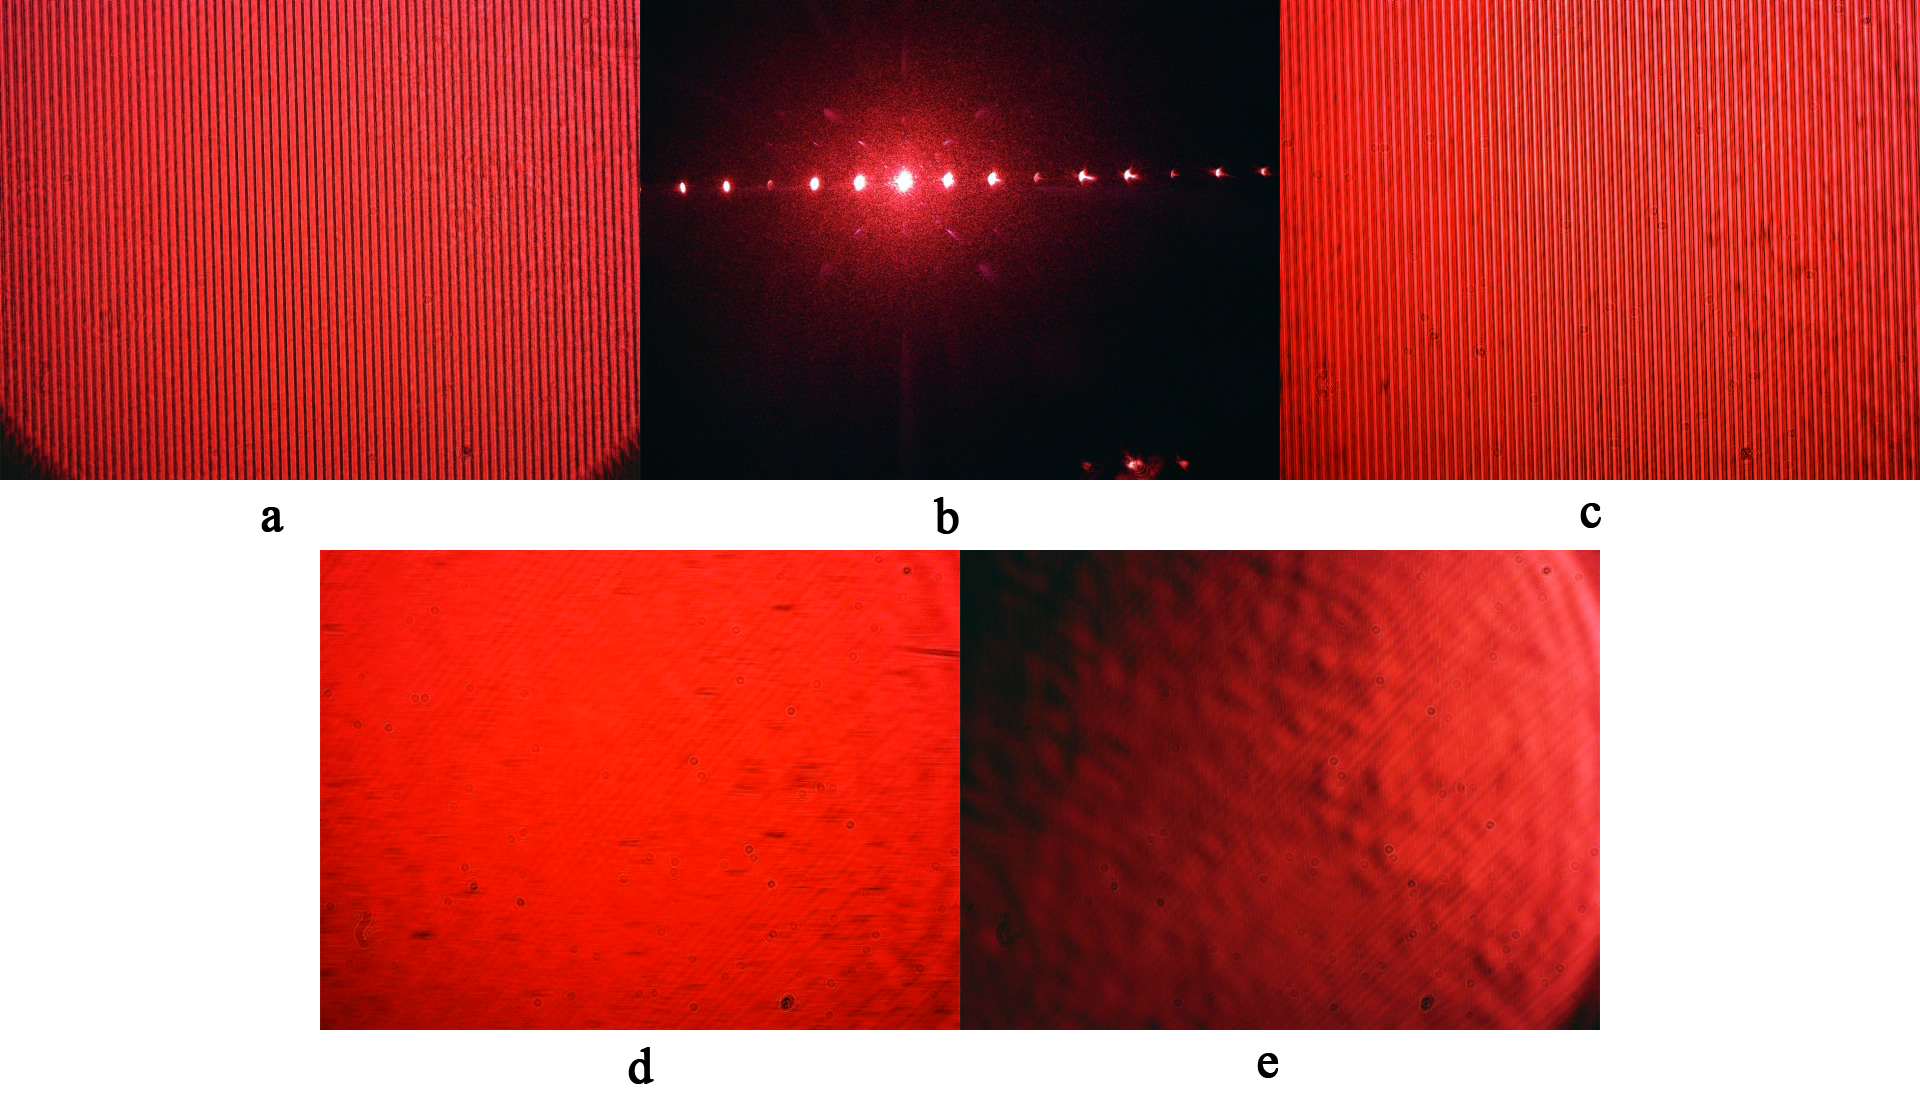
\includegraphics[width=0.8\textwidth]{photos/1d-grating.png}
    \caption{\centering 一维光栅空间频谱与像的分布, a. 像, b. 空间频谱, c. 过横狭缝像面, d. 过竖狭缝像面, e. 过小孔像面}
    \label{fig:experiment3}
\end{figure}

一维光栅的透射函数在水平方向是周期性的, 而在垂直方向是均匀的。当平行光通过该光栅时, 其空间频谱会在傅里叶变换平面(频谱面)上沿水平方向展开, 形成一系列衍射级次(如0级、±1级等), 而竖直方向仅存在零级成分, 因为该方向无周期性变化。横向狭缝保留水平方向的频谱成分, 使像面可见; 竖直狭缝仅通过零频, 导致像面失去周期性结构, 无法观测到光栅的像。小孔在傅里叶光学中相当于一个低通滤波器, 也会导致完全丧失周期性结构。

\subsection{二维光栅空间频谱与像的分布}

\begin{figure}[ht!]
    \centering
    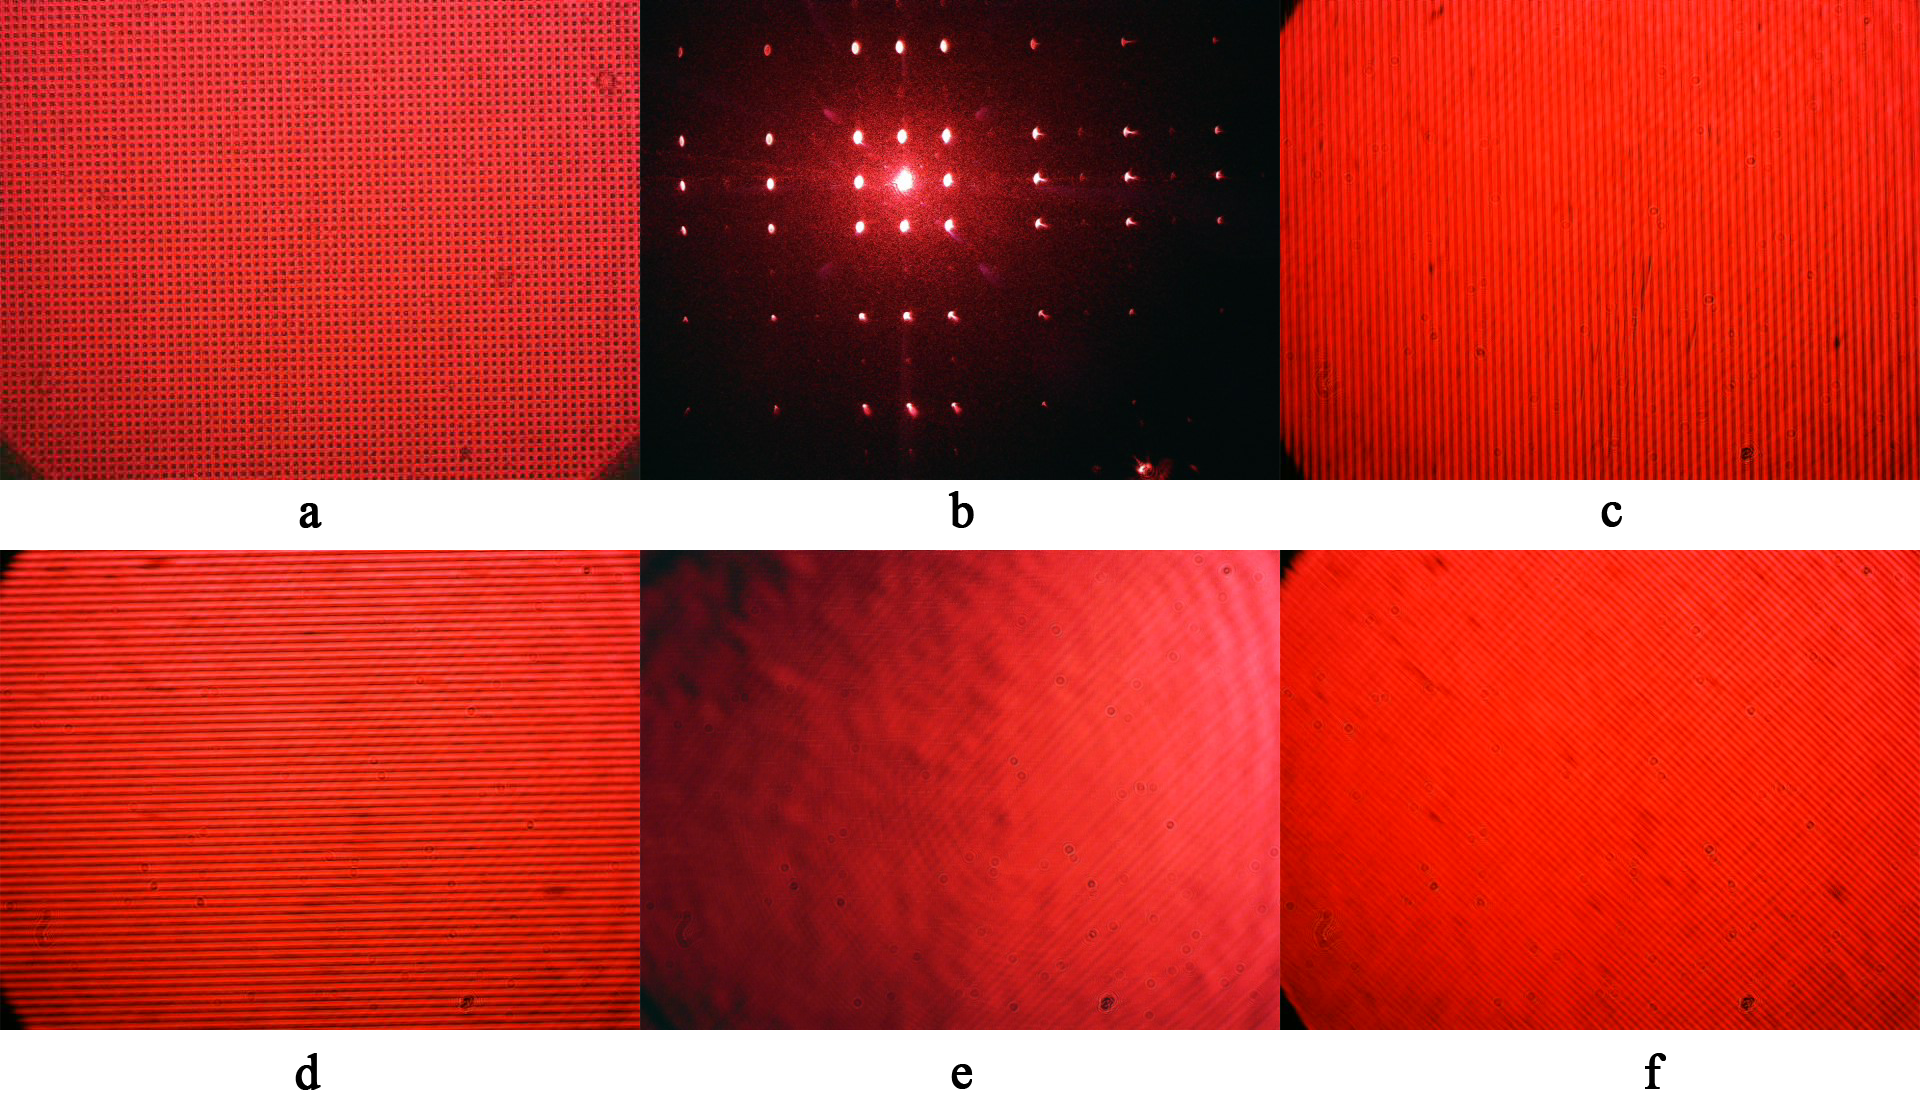
\includegraphics[width=0.8\textwidth]{photos/2d-grating.png}
    \caption{\centering 二维光栅空间频谱与像的分布, a. 像, b. 空间频谱, c. 过横狭缝像面, d. 过竖狭缝像面, e. 过小孔像面, f. 过斜狭缝像面}
    \label{fig:experiment4}
\end{figure}

对于二维光栅而言, 过横狭缝会出现竖条纹, 过竖狭缝会出现横条纹, 均会保留一个方向的信息。小孔会导致周期性结构完全丧失, 而斜狭缝会出现较暗的斜条纹, 这是由于周期性信息的叠加。

\subsection{“光”字样品空间频谱与像的分布}

\begin{figure}[ht!]
    \centering
    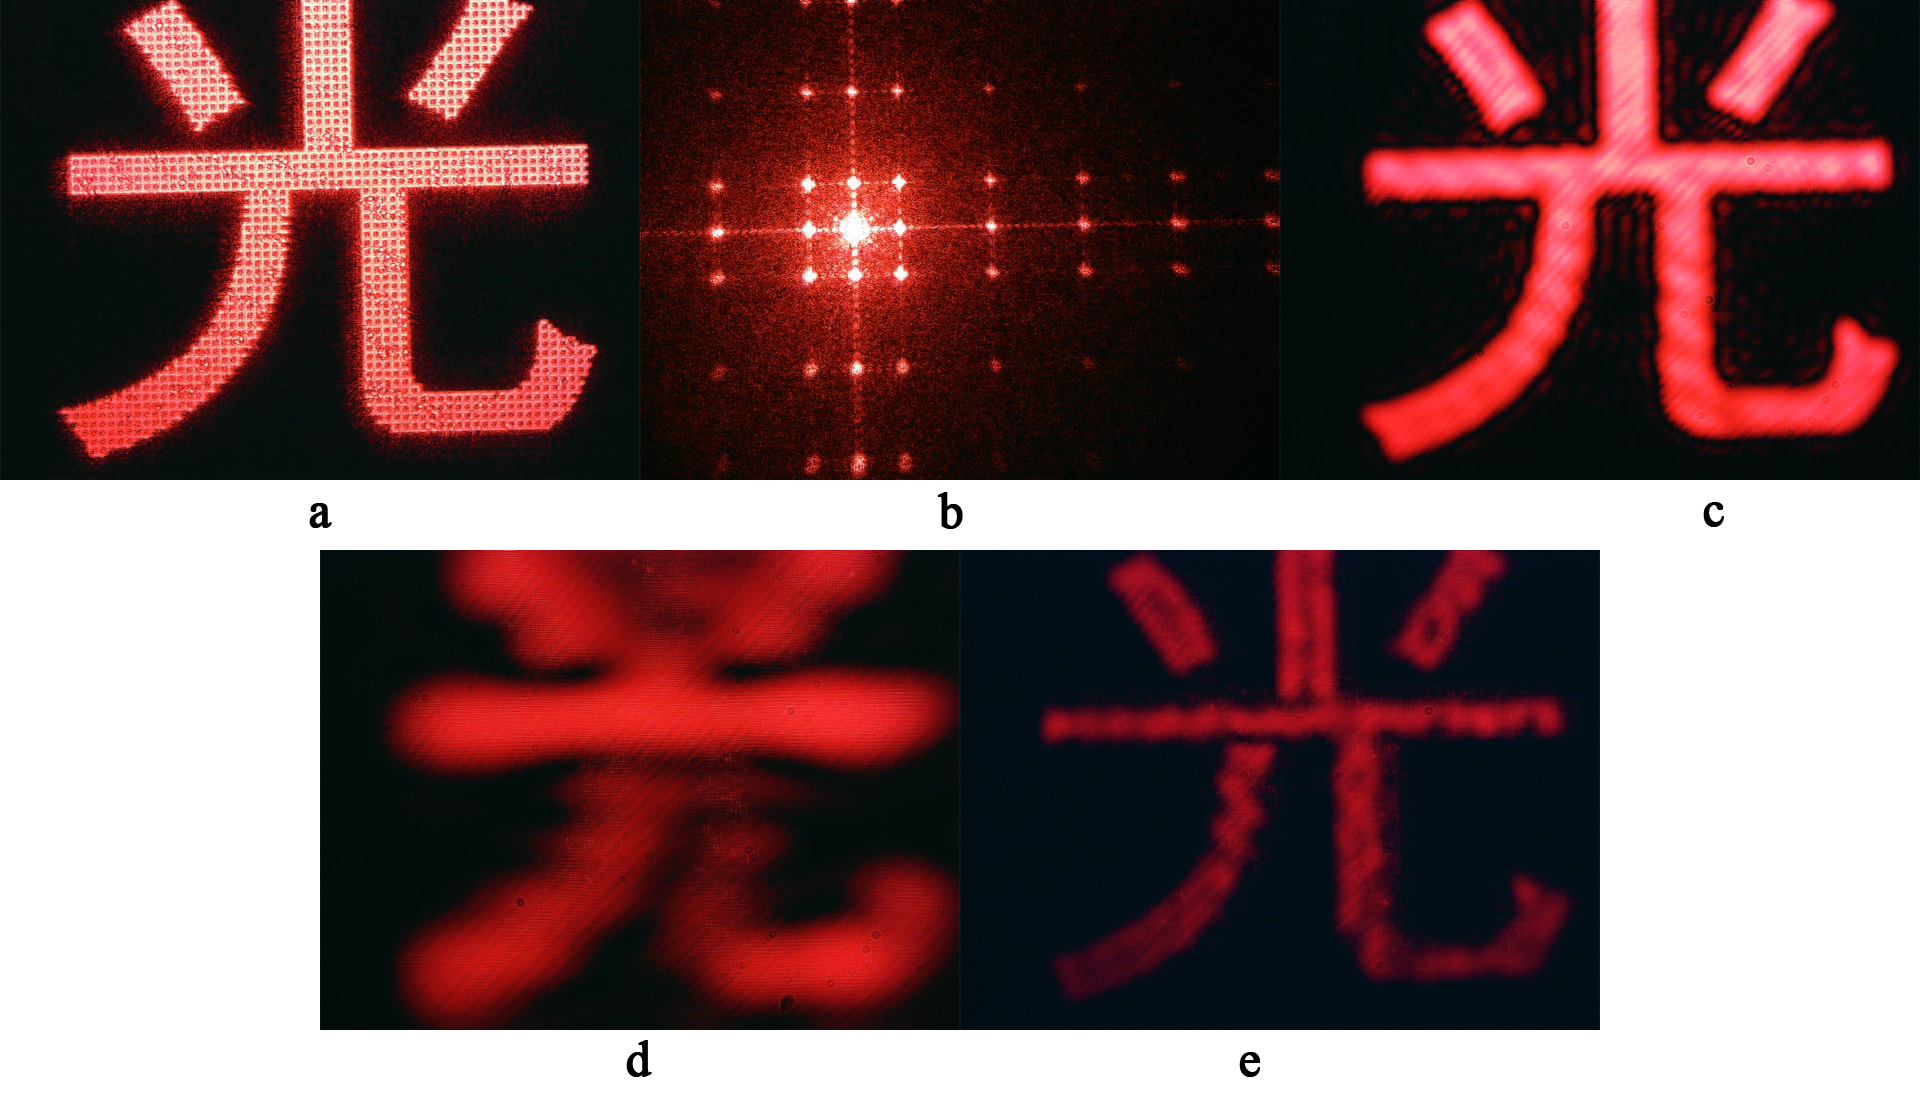
\includegraphics[width=0.8\textwidth]{photos/light.png}
    \caption{\centering “光”字样品空间频谱与像的分布, a. 像, b. 空间频谱, c. 过$\phi=1mm$圆孔光阑像面, d. 过$\phi=0.3mm$圆孔光阑像面, e. 平移光阑使不在光轴上的一个衍射点通过光阑像面}
    \label{fig:experiment5}
\end{figure}

“光”字样品的空间频谱在频谱面上呈现出字样的轮廓, 同时由于字样的边缘有明显的高频成分, 因此频谱面上也有较强的高频成分。通过不同大小的圆孔光阑进行滤波, 可以看到像面的变化, $\phi=1mm$圆孔光阑会导致像面的模糊, 而$\phi=0.3mm$圆孔光阑会导致像面的更加模糊。通过平移光阑, 可以看到“光”字, 但是网格的结构被剔除, 这是由于根据卷积定理, 物体的频谱是光字频谱与网格频谱的卷积, 当光阑在频谱面上选择通过一个非零频的衍射点时, 允许的频谱成分是光字频谱在该点的平移副本。

\subsection{“十”字样品空间频谱与像的分布}

\begin{figure}[h!]
    \centering
    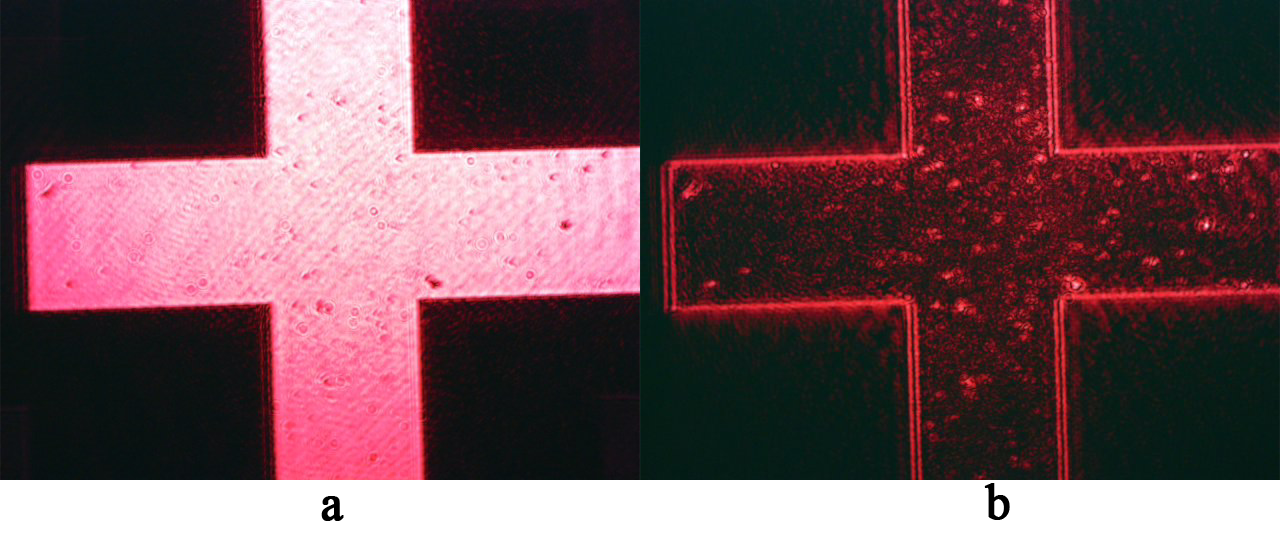
\includegraphics[width=0.8\textwidth]{photos/ten.png}
    \caption{\centering “十”字样品空间频谱与像的分布, a. 像, b. 过圆屏光阑像面}
    \label{fig:experiment6}
\end{figure}

在频谱面上放一圆屏光阑滤去频谱中心部分, 观察到“十”字样品像面上原实心十字的中间区域变暗, 仅保留边缘的亮线, 形成空心十字以及边缘增强的轮廓, 十字线条边缘出现明暗交替的振铃条纹(Gibbs现象)。圆屏光阑滤除中心低频后, 仅允许高频分量通过, 因此无法恢复实心部分(低频分量)的亮度, 导致中间变暗; 保留边缘线条(高频分量)的信息, 形成空心结构。

\subsection{正交光栅的频谱分布}

\begin{figure}[ht!]
    \centering
    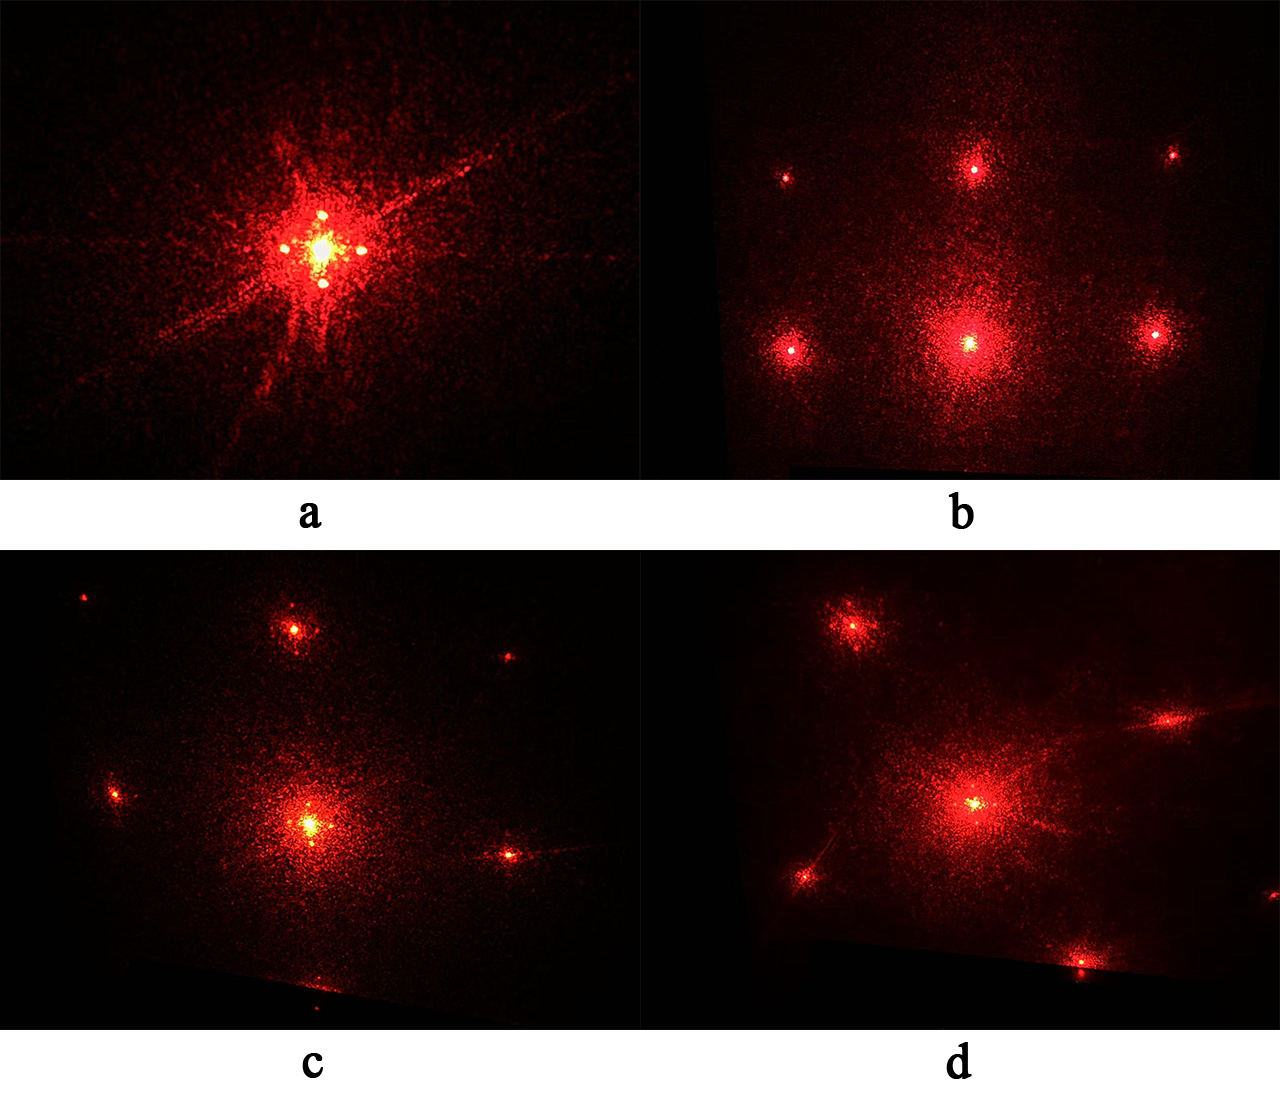
\includegraphics[width=0.6\textwidth]{photos/orthogonal-grating.png}
    \caption{\centering 正交光栅的频谱分布, a. 200条/mm光栅频谱, b. 20条/mm光栅频谱, c. 20条/mm与200条/mm光栅重叠频谱, d. 旋转一条光栅后频谱}
    \label{fig:experiment7}
\end{figure}

20条/mm光栅衍射点靠近频谱面中心(零频点), 相邻衍射级次之间的间距较小, 在频谱面上可见更多衍射点; 200条/mm光栅衍射点分布较为密集, 相邻衍射级次之间的间距较大, 频谱面上衍射点较少。两光栅重叠后, 频谱面上出现了两光栅的频谱叠加, 形成了一系列交叉的频谱点。旋转一条光栅后, 频谱面上的频谱点也随之旋转, 但是频谱点的分布不会发生变化。

\subsection{\texorpdfstring{$\theta$}{theta}调制实验现象}

\begin{figure}[ht!]
    \centering
    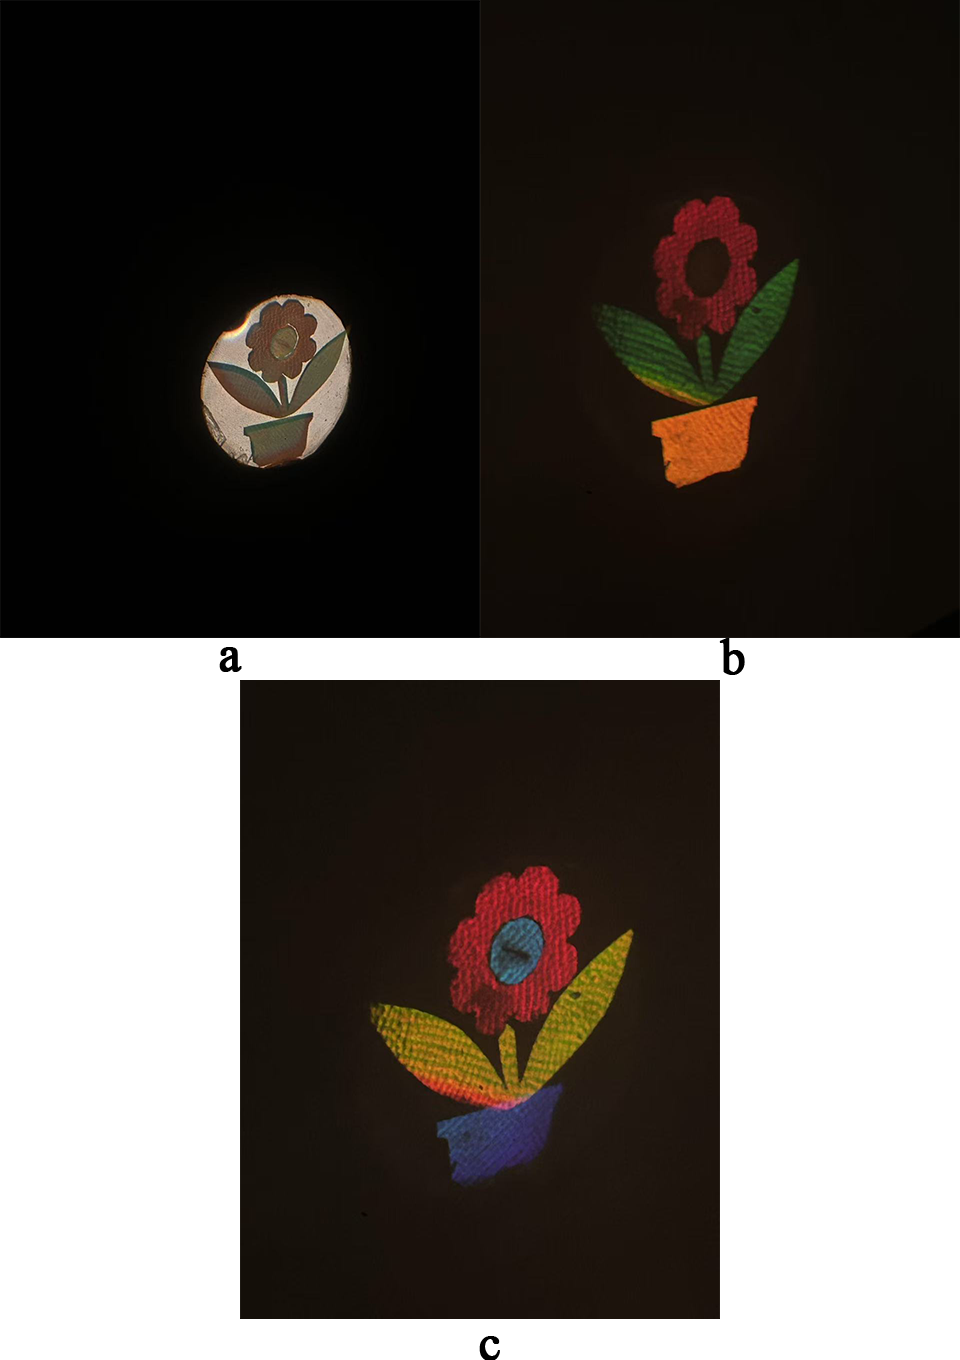
\includegraphics[width=0.4\textwidth]{photos/theta-modulation.png}
    \caption{\centering \texorpdfstring{$\theta$}{theta}调制实验现象, a. 无调制, b. c. 有调制}
    \label{fig:experiment8}
\end{figure}

白光(包含多种波长)照射光栅时, 不同波长的光因衍射角差异($\theta$角)发生色散, 形成光谱分布。通过打开特定衍射点, 可以允许对应频率的光通过, 最终在像平面(花朵位置)重建出预设的颜色分布。

\section{分析与讨论}

\begin{enumerate}
    \item 对于前5个实验, 光路的准直非常重要, 否则会严重影响后续的实验
    \item 对于频谱面上的频谱点, 通过光阑选择不同频率的点, 可以实现频谱的滤波, 从而改变像面的结构
\end{enumerate}

\section{收获与感想}

本次实验通过观察不同结构的样品的频谱和像, 我进一步了解光学傅里叶变换的基本原理, 以及空间频率、空间频谱和空间滤波等相关概念, 对光学成像和光学信息处理有了更深入的了解, 并进一步提升了实验操作的能力。

\end{document}